\section{Preparing the data for network machine learning}
\label{sec:ch2:prepare}
Next, it's time for us to prepare our networks for machine learning algorithms. Like before, you are going to try to capture most of these with functions, because:

\begin{enumerate}
    \item Functions will make the useful data preparation code that we write usable on new networks,
    \item You will gradually build libraries of utility functions,
    \item You can use modularize these functions into other parts of your data pipeline before it gets to your algorithm, to keep a lean module-oriented design,
    \item You can easily try different transformations of the data and evaluate which ones tend to work best.
\end{enumerate}

\subsection{Data cleaning}

Most network machine learning algorithms cannot work with a node which is \emph{isolated}, meaning that the node has no edges. Let's start with fixing this. We can remove isolated nodes from the network as follows:
\begin{enumerate}
\item Compute the number of nodes each node connects to. This consists of summing the matrix along the rows (or columns). The network is undirected, which means that if a node can communicate with another node, that other node can also communicate with that node.
\item Identify any nodes which are connected to zero nodes along either the rows or columns. These are the isolated nodes.
\item Remove the isolated nodes from the adjacency matrix.
\end{enumerate}

Let's see how this works in practice. We begin by first taking the row sums of each node, which tells us how many nodes each node is connected to. Next, we remove all nodes with are not connected to any other nodes (the row and column sum are both zero) from both the adjacency matrix and the labels:

\begin{lstlisting}[style=python]
def remove_isolates(A):
    """
    A function which removes isolated nodes from the 
    adjacency matrix A.
    """
    degree = A.sum(axis=0)  # sum along the rows to obtain the node degree
    out_degree = A.sum(axis=1)
    A_purged = A[~(degree == 0),:]
    A_purged = A_purged[:,~(degree == 0)]
    print("Purging {:d} nodes...".format((degree == 0).sum()))
    return A_purged
    
A = remove_isolates(A)
# Purging 0 nodes...
\end{lstlisting}

So no isolated nodes were found, and consequently no nodes were purged. Great! What else can we do?

A common thing to do with functional MRI connectomes is to, in fact, not look at the correlations themselves, but the absolute correlations. The intuition here is that, if one node is less active when another node is active, that kind of indicates that they are still operating together. Let's take a look at how we can compute the absolute correlations:

\begin{lstlisting}[style=python]
import matplotlib.pyplot as plt
from graphbook_code import heatmap

A_abs = np.abs(A)
fig, axs = plt.subplots(1,3, figsize=(21, 6))
heatmap(A, ax=axs[0], title="Human Connectome, Raw", vmin=np.min(A), vmax=1)
heatmap(A_abs, ax=axs[1], title="Human Connectome, Absolute", vmin=np.min(A), vmax=1)
heatmap(A_abs - A, ax=axs[2], title="Difference(Absolute - Raw)", vmin=0, vmax=1)
\end{lstlisting}

Several of the values will change (the faint bands), which is indicated by larger differences from the raw to the absolute data. You can use this \texttt{heatmap} function to plot the adjacency matrix as you manipulate it later on in this section.

To streamline the process of cleaning up the raw data, you will often need to write custom data cleaners. You will want your cleaners to work seamlessly with \texttt{sklearn}'s functions, such as pipelines, and will require you to only implement three class methods: \texttt{fit()}, \texttt{transform()}, and \texttt{fit\_transform()}. By adding \texttt{TransformerMixin} as a base class, we do not even have to implement the third one! If we use \texttt{BaseEstimator} as a base class, we will also obtain \texttt{get\_params()} and \texttt{set\_params()}, which will be useful for hyperparameter tuning steps you might need in other settings. 

Here is an example cleaner class which purges the adjacency matrix of isolates and remaps the categorical labels to numbers. A key step to implementing this all as cleanly as possible is that the inputs, an adjacency matrix and a vector of node labels, are passed in as a \emph{single} tuple object. This is because \texttt{sklearn} anticipates that the return arguments from calls of \texttt{transform()} can be passed sequentially to one another.

\begin{lstlisting}[style=python]
from sklearn.base import TransformerMixin, BaseEstimator

class CleanData(BaseEstimator, TransformerMixin):

    def fit(self, X):
        return self

    def transform(self, X):
        print("Cleaning data...")
        Acleaned = remove_isolates(X)
        A_abs_cl = np.abs(Acleaned)
        self.A_ = A_abs_cl
        return self.A_

data_cleaner = CleanData()
A_clean = data_cleaner.transform(A)
# Cleaning data...
# Purging 0 nodes...
\end{lstlisting}

\subsection{Edge weight transformations}

One of the most important transformations that we will come across in network machine learning is called \emph{edge-weight transformation}. Many networks you enounter, such as the human diffusion connectome, will have edge weights which do not just take values of 1 or 0 (edge or no edge, a \emph{binary} network); rather, many networks may have discrete-weighted edges (the edges take non-negative inter values, such as 0, 1, 2, 3, ...), or decimal-weight edges (the edges take values like 0, 0.1234, 0.234, 2.4234, ...). For a number of reasons discussed in Section \ref{sec:ch4:regularization}, this is often not really a desirable characteristic.  The edges in a network might be error prone, and it might only be desirable to capture one (or a few) properties about the edge weights, rather than just leave them in their raw values. Further, a lot of the techniques we come across throughout this book might not work on networks which are not binary. For this reason, we need to get accustomed to transforming the edge weights to take new sets of values.

There are two common approaches to transform edge weights: the first is called binarization (set all of the edges to take a value of 0 or 1), and the second is called an ordinal transformation. 

\subsubsection*{Binarization of edges} 

Binarization is quite simple. It means the edges in the raw network take non-binary values (values other than just 0s and 1s), and you need them to be 0s and 1s for your algorithm. How do you solve this? 

The simplest thing to do is usually to just look at which edges take a value of zero, and keep them as zero, and then set all of the edges which take a non-zero value to one. Let's take a look at how we can implement this using \texttt{graspologic}. We first look at the network before binarization, and then after:

\begin{lstlisting}[style=python]
from graspologic.utils import binarize

threshold = 0.4
A_bin = binarize(A_clean > threshold)
\end{lstlisting}

If you plot the cleaned adjacency matrix and the binarized adjacency matrix like in Figure \ref{fig:ch2:cleaned_connectomes}, you will see that it retains a lot of the ``general idea'' of the weighted adjacency matrix, but it's a lot simpler. Whereas the edge weights in the left plot were \emph{continuous}, we've now \emph{binarized} the edges of the network to only take two possible values ($0$ or $1$). This has the effect of potentially reducing the variance (since we no longer will need as complicated of descriptions to summarize the edge-weights), but potentially increasing the bias (since we have simplified our data and have therefore potentially "thrown away" information that might be important).

Another way we could have normalized these edge weights is through something called a \emph{pass to ranks}. Through a pass to ranks, the edge weights are discarded entirely, with one exception: the edges which are non-zero are first ranked, from smallest to largest, with the largest item having a rank of one, and the smallest item having a rank of 1/(number of non-zero edges). This is called an \emph{ordinal transformation}, in that it preserves the \emph{orders} of the edge-weights, but discards all other information. The adjacency matrix of the ranked connectome is shown in Figure \ref{fig:ch2:cleaned_connectomes}(C).

\begin{lstlisting}[style=python]
from graspologic.utils import pass_to_ranks

A_ptr = pass_to_ranks(A_clean)
\end{lstlisting}
\begin{figure}[h]
    \centering
    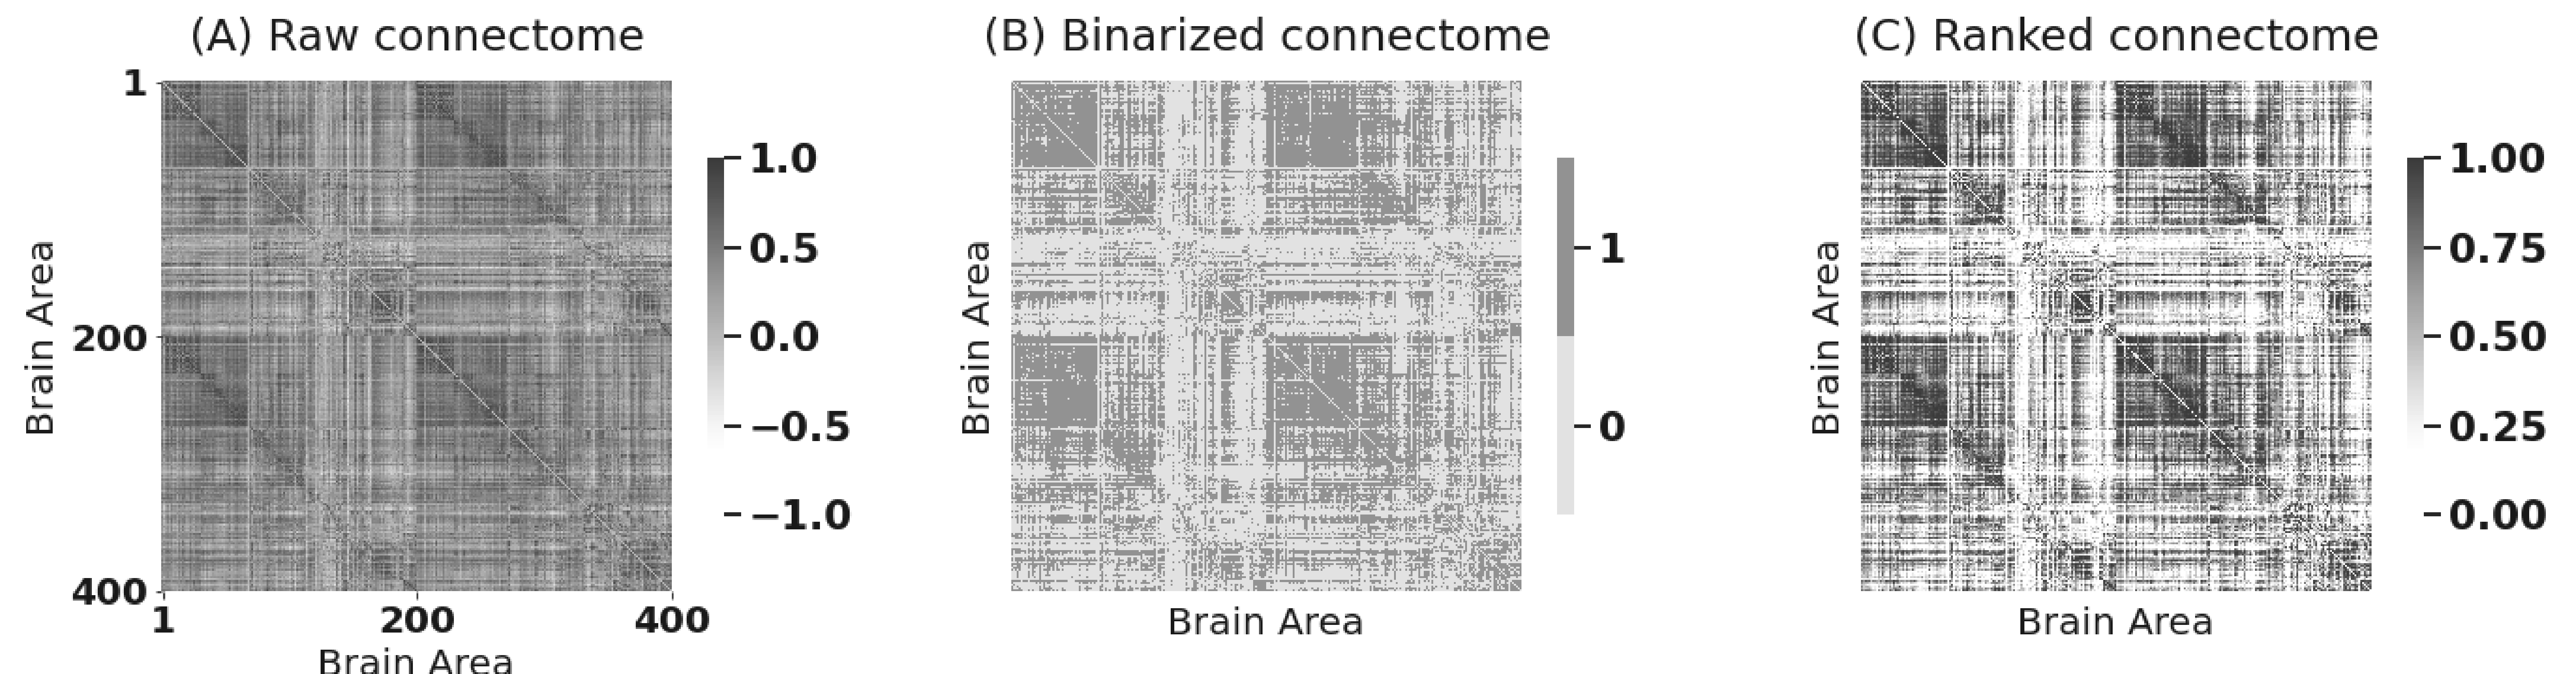
\includegraphics[width=\linewidth]{foundations/ch2/Images/cleaning_connectomes.png}
    \caption[Re-weighting connectome edge-weights]{\textbf{(A)} The cleaned connectome, before re-weighting. \textbf{(B)} The binarized connectome. \textbf{(C)} The ranked connectome.}
    \label{fig:ch2:cleaned_connectomes}
\end{figure}

This has shifted the histogram of edge-weights, as we can see by plotting a histogram:

\begin{lstlisting}[style=python]
import seaborn as sns

fig, ax = plt.subplots(2,1, figsize=(10, 10))
sns.histplot(A_clean[A_clean > 0].flatten(), ax=ax[0]);
ax[0].set_xlabel("Edge weight")
ax[0].set_title("Histogram of human connectome, non-zero edge weights");

sns.histplot(A_ptr[A_ptr > 0].flatten(), ax=ax[1]);
ax[1].set_xlabel("ptr(Edge weight)")
ax[1].set_title("Histogram of human connectome, passed-to-ranks")
\end{lstlisting}
The histograms before and after passing the adjacency matrix to ranks are shown in Figure \ref{fig:ch2:ptrhists}.

\begin{figure}[h]
    \centering
    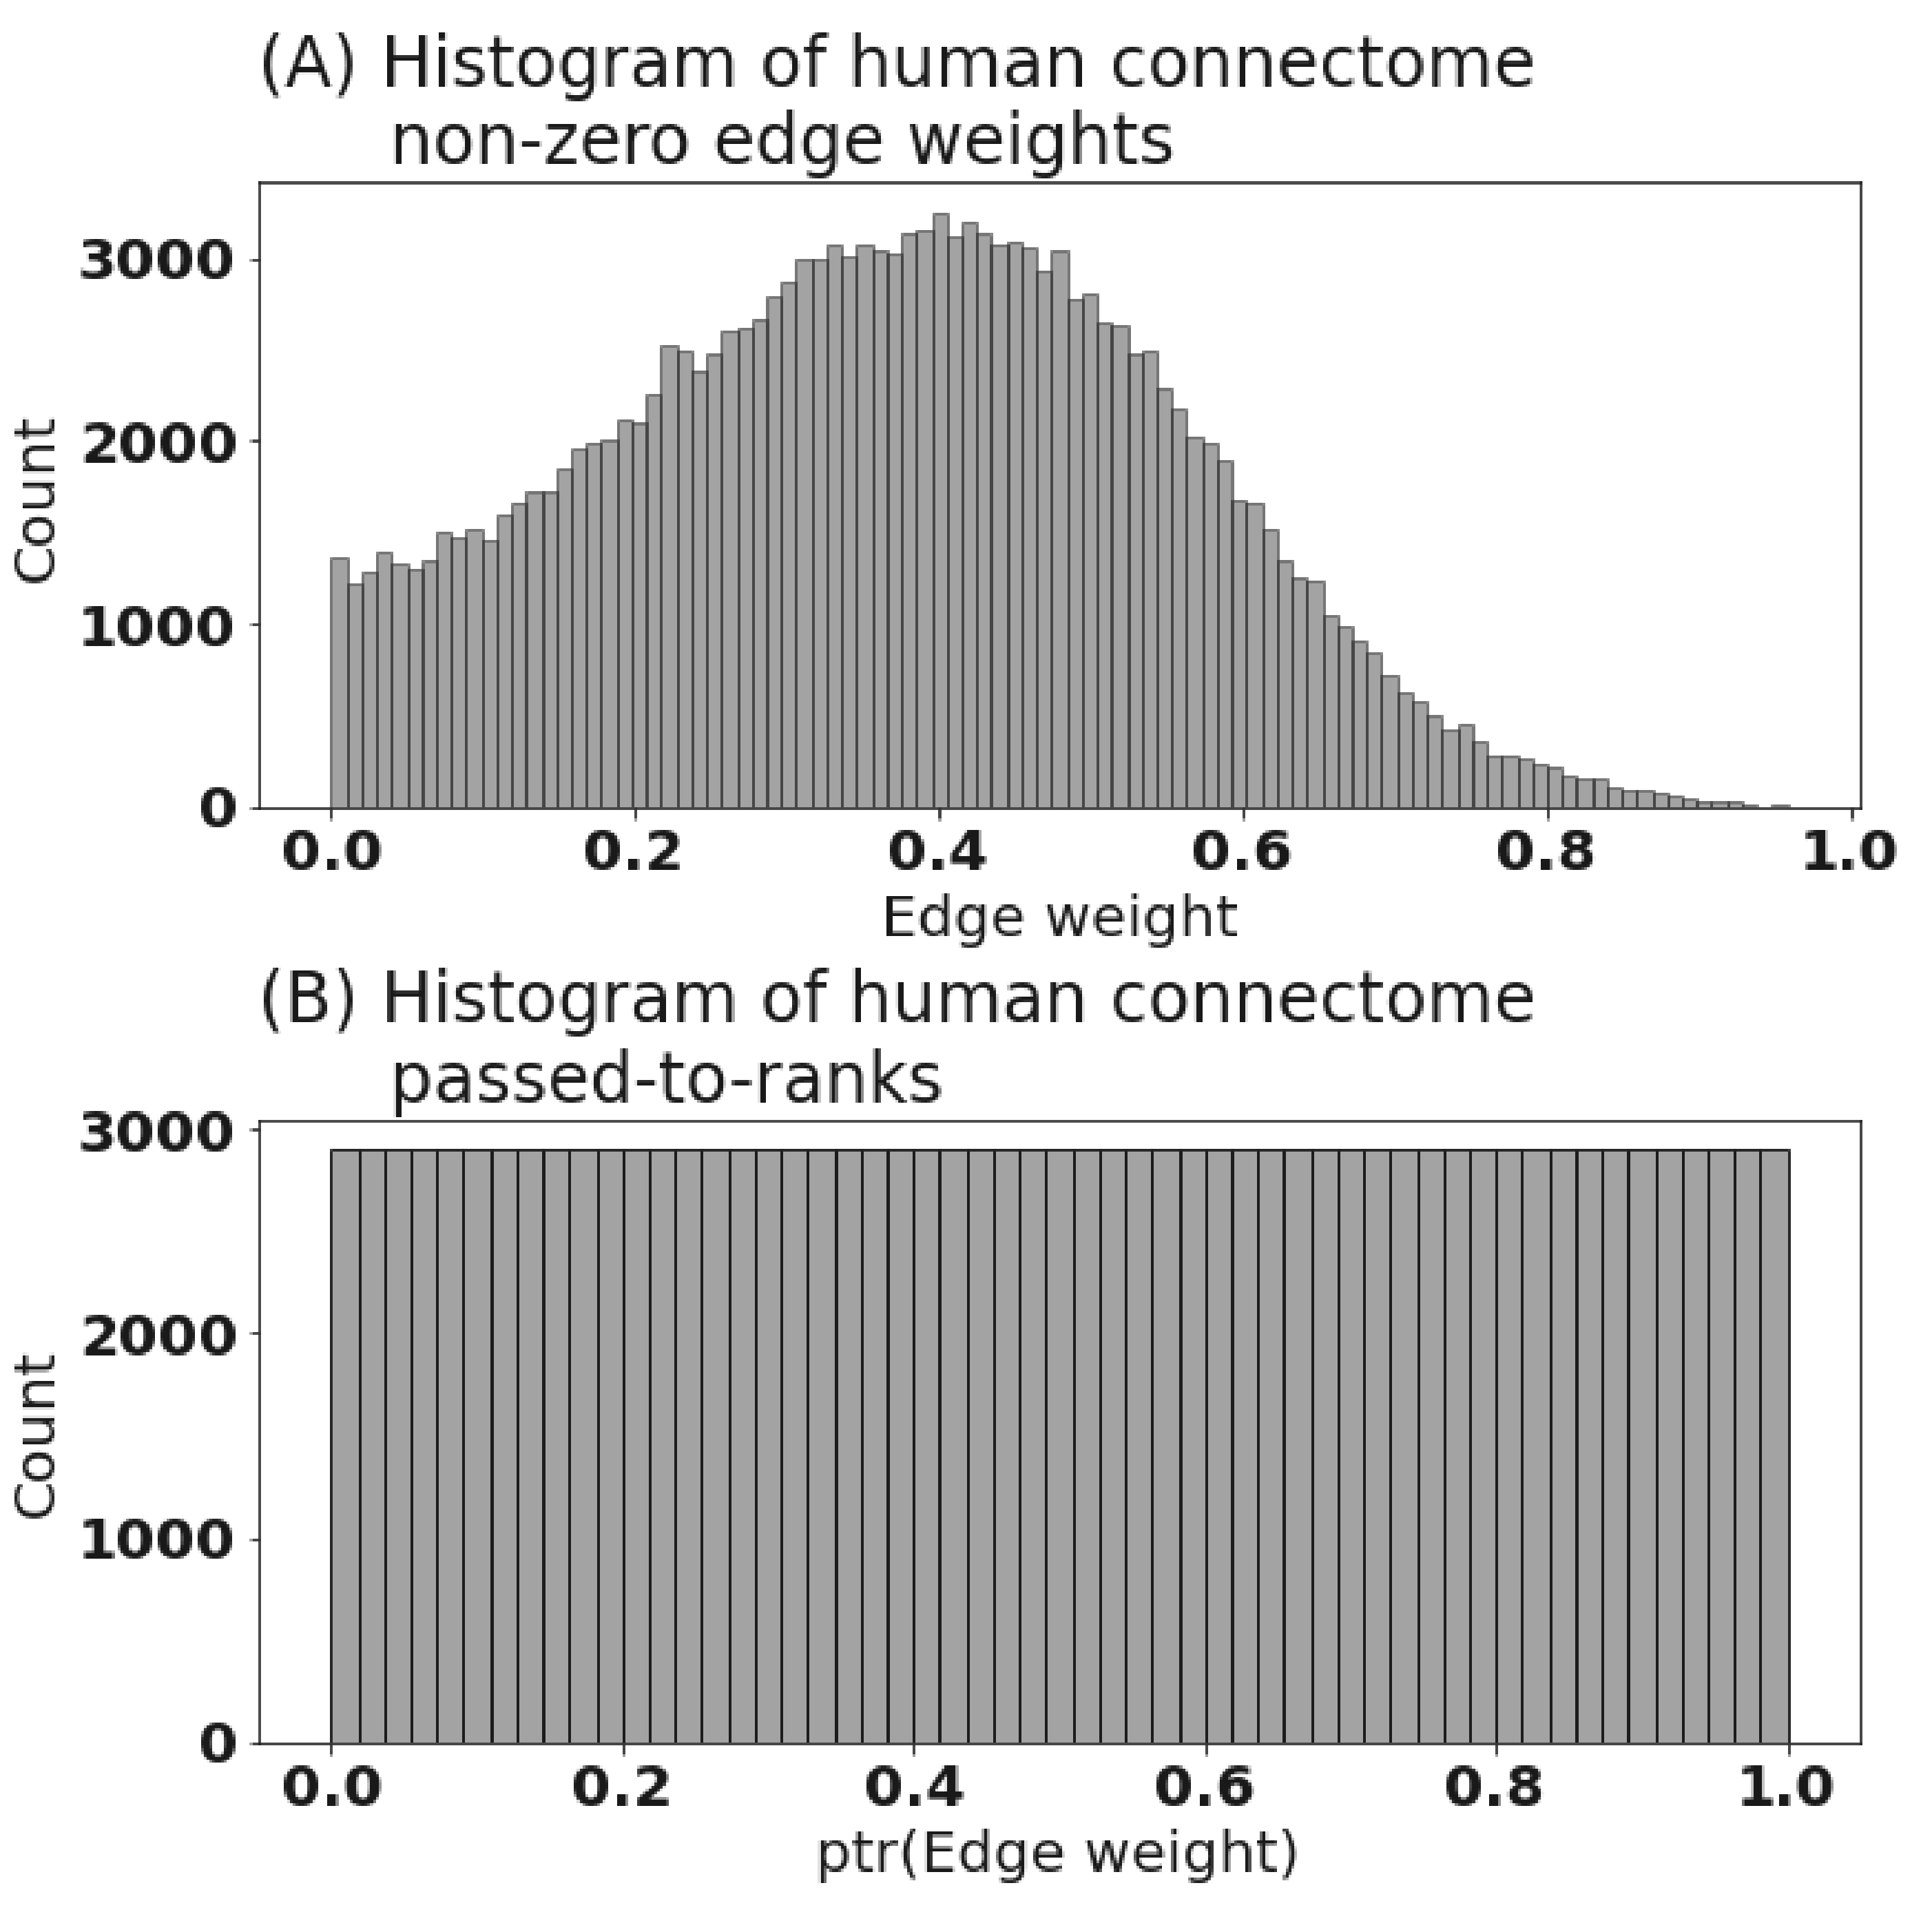
\includegraphics[width=0.6\linewidth]{foundations/ch2/Images/ptrhists.png}
    \caption[Histograms of connectome edge weights]{\textbf{(A)} Histogram of the edge-weights in the adjacency matrix before normalization. \textbf{(B)} Histogram of the edge weights in the adjacency matrix after \texttt{ptr}.}
    \label{fig:ch2:ptrhists}
\end{figure}

This has the desirable property that it bounds the network's edge weights to be between $0$ and $1$, as we can see above, which is often crucial if we seek to compare two or more networks and the edge weights are relative in magnitude (an edge's weight might mean something in relation to another edge's weight in that same network, but an edge's weight means nothing in relation to another edge's weight in a separate network). Further, passing to ranks is not very susceptible to outliers, as we will see in later chapters. 

Again, we will turn the edge-weight transformation step into its own class:

\begin{lstlisting}[style=python]
class FeatureScaler(BaseEstimator, TransformerMixin):
    
    def fit(self, X):
        return self
    
    def transform(self, X):
        print("Scaling edge-weights...")
        A_scaled = pass_to_ranks(X)
        return (A_scaled)
    
feature_scaler = FeatureScaler()
A_cleaned_scaled = feature_scaler.transform(A_clean)
# Scaling edge-weights...
\end{lstlisting}

\subsubsection*{Transformation pipelines}

As you can see, there are a number of data transformations that need to be executed to prepare network data for machine learning algorithms. One thing that might be desirable is to develop a pipeline which automates the data preparation process for you. We perform this using the \texttt{Pipeline} class from \texttt{sklearn}. The \texttt{Pipeline} class can help us apply sequences of transformations. Here is a simple pipeline for doing all of the steps we have performed so far:
\begin{lstlisting}[style=python]
from sklearn.pipeline import Pipeline

num_pipeline = Pipeline([
    ('cleaner', CleanData()),
    ('scaler', FeatureScaler()),
])

A_xfm = num_pipeline.fit_transform(A)
# Cleaning data...
# Purging 0 nodes...
# Scaling edge-weights..
\end{lstlisting}

The pipeline class takes a list of name/estimator pairs defining a sequence of steps. All but the last estimator must be transformers, which implement the \texttt{fit\_transform()} method. In our case, this is handled directly by the \texttt{TransformerMixin} base class.

When you call the \texttt{fit\_transform()} method of the numerical pipeline, it calls the \texttt{fit\_transform()} method on each of the transformers, and passes the output of each call as the parameter to the next call, until it reaches the final estimator, for which it just calls the \texttt{fit()} method. 

Next, we'll see the real handiness of the \texttt{Pipeline} module. The reason we went to lengths to define a pipeline was that we wanted to have an easily reproducible procedure that we could efficiently apply to new connectomes. This is easy to apply to the second subject in our dataset:

\begin{lstlisting}[style=python]
A_xfm2 = num_pipeline.fit_transform(As[1])
# Cleaning data...
# Purging 0 nodes...
# Scaling edge-weights...
\end{lstlisting}

\newpage